%%%%%%%%%%%%%%%%%%%%%%%%%%%%%%%%%%%%%%%%%%%%%%%%%%%%%%%%%%%%%%%%%%%%%%
% Edit the title below to update the display in My Documents
%\title{Project Report}
%
%%% Preamble
\documentclass[paper=a4, fontsize=12pt]{scrartcl}
\usepackage[T1]{fontenc}
\usepackage{fourier}

\usepackage[czech]{babel}
\usepackage[utf8]{inputenc}									
\usepackage[protrusion=true,expansion=true]{microtype}	
\usepackage{amsmath,amsfonts,amsthm} % Math packages
\usepackage[pdftex]{graphicx}
\usepackage{subfig}	
\usepackage{url}
\usepackage[table,xcdraw]{xcolor}
\usepackage{float}

%%% Custom sectioning
\usepackage{sectsty}
\allsectionsfont{\centering \normalfont\scshape}


%%% Custom headers/footers (fancyhdr package)
\usepackage{fancyhdr}
\pagestyle{fancyplain}
\fancyhead{}											% No page header
\fancyfoot[L]{}											% Empty 
\fancyfoot[C]{}											% Empty
\fancyfoot[R]{\thepage}									% Pagenumbering
\renewcommand{\headrulewidth}{0pt}			% Remove header underlines
\renewcommand{\footrulewidth}{0pt}				% Remove footer underlines
\setlength{\headheight}{13.6pt}


%%% Equation and float numbering
\numberwithin{equation}{section}		% Equationnumbering: section.eq#
\numberwithin{figure}{section}			% Figurenumbering: section.fig#
\numberwithin{table}{section}				% Tablenumbering: section.tab#


%%% Maketitle metadata
\newcommand{\horrule}[1]{\rule{\linewidth}{#1}} 	% Horizontal rule

\title{
		%\vspace{-1in} 	
		\usefont{OT1}{bch}{b}{n}
		\normalfont \normalsize \textsc{Fakulta informačních technológií ČVUT} \\ [25pt]
		\horrule{0.5pt} \\[0.4cm]
		\huge BI-PST Domácí úkol \\
		\horrule{2pt} \\[0.5cm]
}
\author{
		\normalfont 								\normalsize
        Patrik Jantošovič\\[-3pt]		\normalsize
        Tomáš Zvara\\[-3pt]		\normalsize
        Tomáš Janecký\\[-3pt]		\normalsize
        \today
}
\date{}


%%% Begin document
\begin{document}
\maketitle
\section{Parametry a datový soubor}
Reprezentant: Patrik Jantošovič\\
K = den narození = 16\\
L = počet písmen v příjmení = 10\\
M = ((K+L)*46)mod11 + 1 = 2\\
Výsledkem je tedy datový soubor: case0102, mzda dle pohlaví\\

\subsection{Vytvoření datového souboru}
Řešení úloh předpokladá úspěšnou instalaci knihovni Sleuth2 a vytvoření .csv souboru s příslušnými daty.\\
Postup uvedeme jednou na začátku abychom jsme se neopakovali.

\begin{itemize}
	\item >> install.packages("Sleuth2")
		\begin{itemize}
		\item Instalace package Sleuth2 
		\end{itemize}
	\item >> library(Sleuth2)
		\begin{itemize}
		\item Načítaní package Sleuth2 
		\end{itemize}
	\item >> write.table(case0102,"C:/data.csv",row.names=F,sep=";",dec=",")
		\begin{itemize}
		\item Zápis dat do .csv souboru
		\end{itemize}
\end{itemize}

\section{Řešení úkolú}
\subsection{Úkol číslo 1}
(1b) Načtěte datový soubor a rozdělte sledovanou proměnnou na příslušné dvě pozorované skupiny. Data stručně popište. 
Pro každu skupinu zvlášť odhadněte střední hodnotu, rozptyl a medián příslušného rozdělení.

\begin{itemize}
	\item >> data<-read.table("C:/data.csv",header=TRUE,sep=";")
		\begin{itemize}
		\item Načteme data z připraveného souboru
		\end{itemize}
	\item >> female<-data[1:61,]
		\begin{itemize}
		\item Načítaní dat pro pozorovanou skupinu: Female
		\end{itemize}
	\item >> male<-data[62:93,]
		\begin{itemize}
		\item Načítaní dat pro pozorovanou skupinu: Male
		\end{itemize}
	\item >> female<-female[,1]
		\begin{itemize}
		\item Odřiznutí sloupce s pohlavím pro pozorovanou skupinu: Female
		\end{itemize}
	\item >> male<-male[,1]
		\begin{itemize}
		\item Odřiznutí sloupce s pohlavím pro pozorovanou skupinu: Male
		\end{itemize}
	\item >> length(male)
		\begin{itemize}
		\item Velikost dat pro pozorovanou skupinu: Male
		\end{itemize}
	\item >> length(female)
		\begin{itemize}
		\item Velikost dat pro pozorovanou skupinu: Female
		\end{itemize}
	\item >> var(male)
		\begin{itemize}
		\item Rozptyl pro pozorovanou skupinu: Male
		\end{itemize}
	\item >> var(female)
		\begin{itemize}
		\item Rozptyl pro pozorovanou skupinu: Female
		\end{itemize}
	\item >> mean(male)
		\begin{itemize}
		\item Střední hodnota pro pozorovanou skupinu: Male
		\end{itemize}
	\item >> mean(female)
		\begin{itemize}
		\item Střední hodnota pro pozorovanou skupinu: Female
		\end{itemize}
	\item >> median(male)
		\begin{itemize}
		\item Medián pro pozorovanou skupinu: Male
		\end{itemize}
	\item >> median(female)
		\begin{itemize}
		\item Medián pro pozorovanou skupinu: Female
		\end{itemize}
\end{itemize}
Výsledky zapíšeme do následujíci tabulky:\\
\begin{table}[htb]
\begin{tabular}{lllll}
\rowcolor[HTML]{EFEFEF}
Pohlaví & Velkost dat & Střední hodnota & Rozptyl & Medián \\
\cellcolor[HTML]{EFEFEF}Male     &     32       &         5956.875        &   477112.5      &   6000     \\
\cellcolor[HTML]{EFEFEF}Female   &      61       &         5138.852        &    291460.3     &   5220    
\end{tabular}
\end{table}

\subsection{Úkol číslo 2}
(1b) Pro každou skupinu zvlášť odhadněte hustotu a distribuční funkci pomocí histogramu a empirické distribuční funkce.

\begin{itemize}
	\item >> hist(female, freq=FALSE)
		\begin{itemize}
		\item Vykreslení histogramu female. freq=FALSE používame jako přepínač pro hustotu
		\end{itemize}
	\item >>hist(male, freq=FALSE)
		\begin{itemize}
	        \item Vykreslení histogramu female. freq=FALSE používame jako přepínač pro hustotu
		\end{itemize}
	\item >>plot(density(male))
		\begin{itemize}
		\item Vykreslení hustoty Male
		\end{itemize}
	\item >>plot(density(female))
		\begin{itemize}
		\item Vykreslení hustoty Female
		\end{itemize}
	\item >>plot(ecdf(male))
		\begin{itemize}
		\item Vykreslení empirické distribuční funkce pro Male
		\end{itemize}
	\item >>plot(ecdf(female))
		\begin{itemize}
		\item Vykreslení empirické distribuční funkce pro Female
		\end{itemize}
\end{itemize}
Výsledkem jsou grafy přiložené na následující stránce.%
\begin{figure}[H]%
    \centering
    \subfloat[Male]{{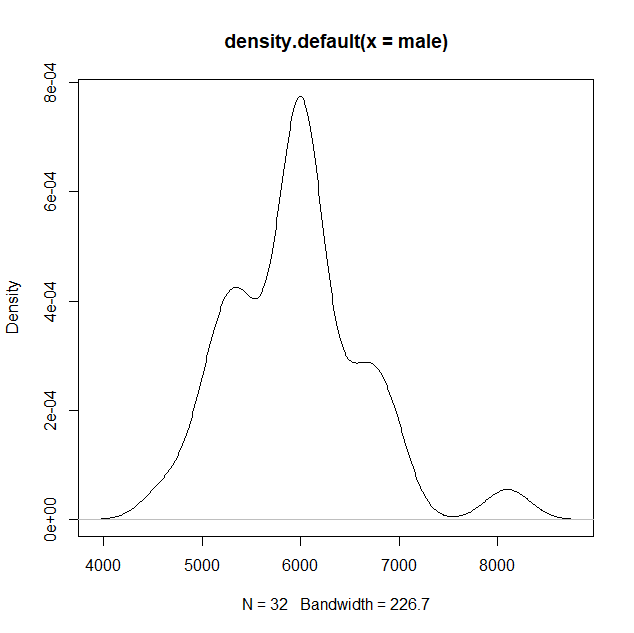
\includegraphics[width=0.4\textwidth]{hustota-male.png} }}%
    \qquad
    \subfloat[Female]{{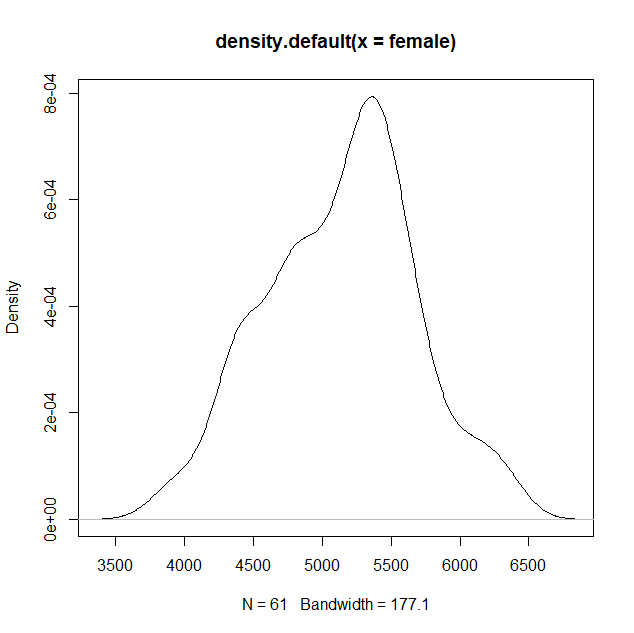
\includegraphics[width=0.4\textwidth]{hustota-female.png} }}%
    \caption{Hustota}%
    \label{fig:example}%
\end{figure}
\begin{figure}[H]%
    \centering
    \subfloat[Male]{{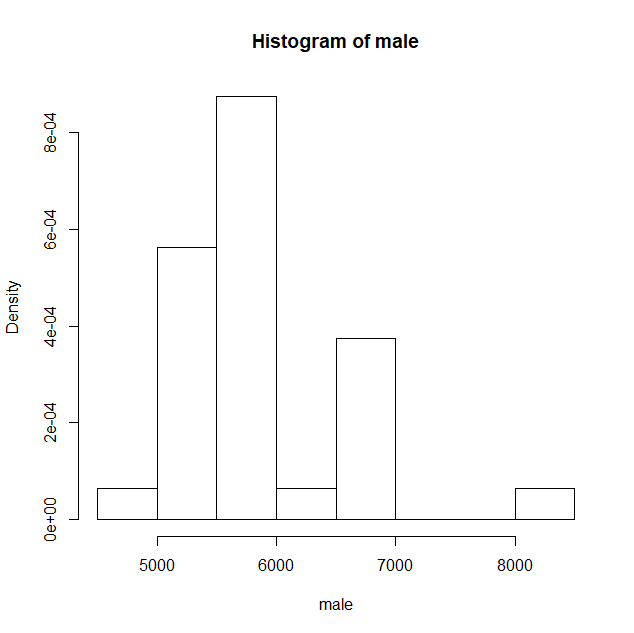
\includegraphics[width=0.4\textwidth]{histogram-male.png} }}%
    \qquad
    \subfloat[Female]{{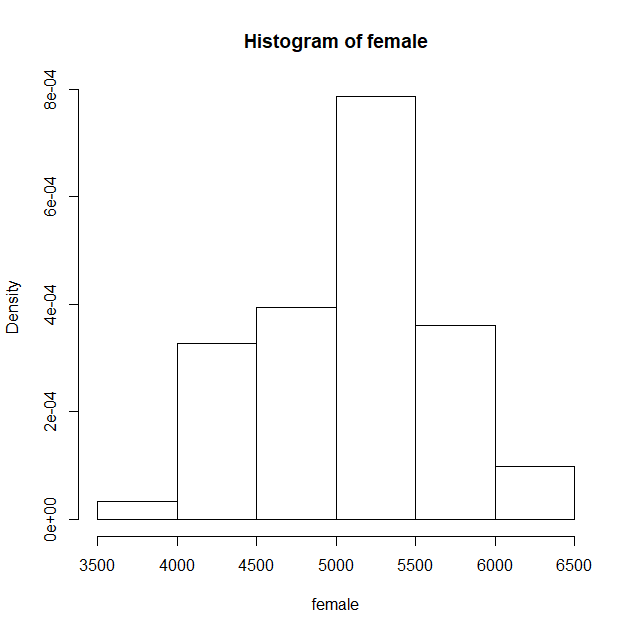
\includegraphics[width=0.4\textwidth]{histogram-female.png} }}%
    \caption{Histogram}%
    \label{fig:example}%
\end{figure}
\begin{figure}[H]%
    \centering
    \subfloat[Male]{{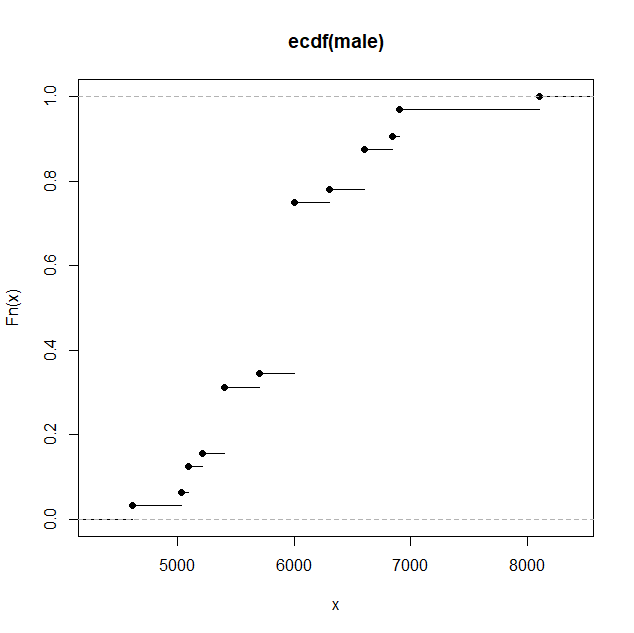
\includegraphics[width=0.4\textwidth]{ecdf-male.png} }}%
    \qquad
    \subfloat[Female]{{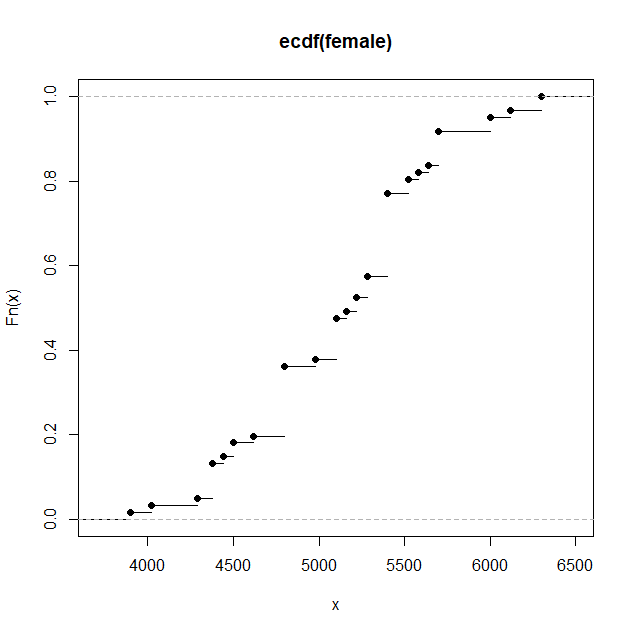
\includegraphics[width=0.4\textwidth]{ecdf-female.png} }}%
    \caption{Empirická distribuční funkce}%
    \label{fig:example}%
\end{figure}

\subsection{Úkol číslo 3}
(3b) Pro každou skupinu zvlášť najděte nejbližší rozdělení: Odhadněte parametry normálního, exponenciálního a rovnoměrného rozdělení. 
Zaneste příslušné hustoty s odhadnutými parametry do grafů histogramu. Diskutujte, které z rozdělení odpovídá pozorovaným datům nejlépe.
\begin{itemize}
	\item Male
		\begin{itemize}
		\item  >> hist(male, freq=FALSE)
		        \begin{itemize}
		        \item Porovnávame distribuční funkce různých rozdělení na histogramu.
		        \end{itemize}
		\item Normální rozdělení
			\begin{itemize}
		        \item >> maleV<-seq(min(male),max(male),10)
		                \begin{itemize}
		                \item vytvoříme si sekvenci hodnot od nejmenší po největší hodnoty 
		                \end{itemize}
		        \item >> maleNorm<-dnorm(maleV, mean = mean(male), sd = sd(male))
		                \begin{itemize}
		                \item využijeme funkci dnorm na převod pro body normálního rozdělení
		                \end{itemize}
		        \item >> lines(maleV,maleNorm, col=''blue'')
		                \begin{itemize}
		                \item vykreslíme normální rozdělení na histogram
		                \end{itemize}
		        \end{itemize}
		\item Exponenciální rozdělení
			\begin{itemize}
		        \item >> lambdaMale<-1/mean(male)
		                \begin{itemize}
		                \item vypočteme si parametr pro exponenciální rozdělení jako $\frac{1}{střední \ hodnota}$
		                \end{itemize}
		        \item >> maleExp<-dexp(maleV, lambdaMale)
		                \begin{itemize}
		                \item využijeme funkci dexp na vypočet bodu exponenciálního rozdělení
		                \end{itemize}
		        \item >>  lines(maleV,maleExp, col=''red'')
		                \begin{itemize}
		                \item vykreslíme exponencionální rozdělení na histogram
		                \end{itemize}
		        \end{itemize}
		\item Uniformní rozdělení
			\begin{itemize}
		        \item >> aMale<-mean(male)-sqrt(3*var(male))
		        \item >> bMale<-sqrt(3*var(male))+mean(male)
		                \begin{itemize}
		                \item vypočteme si parametr `a` a `b` pro uniformní rozdělení podle vztahu k střední hodnote a rozptylu ze cvičení
		                \end{itemize}
		        \item >> maleUnif<-dunif(maleV, aMale,bMale)
		                \begin{itemize}
		                \item využijeme funkci dunif na výpočet bodu uniformního rozdělení
		                \end{itemize}
		        \item >> lines(maleV,maleUnif, col=''yellow'')
		                \begin{itemize}
		                \item vykreslíme uniformní rozdělení na histogram
		                \end{itemize}
		        \end{itemize}
		\end{itemize}
	\item Female
		\begin{itemize}
		\item  >> hist(female, freq=FALSE)
		        \begin{itemize}
		        \item Porovnávame distribuční funkce různých rozdělení na histogramu.
		        \end{itemize}
		\item Normálni rozdělení
			\begin{itemize}
		        \item >> femaleV<-seq(min(female),max(female),10)
		                \begin{itemize}
		                \item vytvoříme si sekvenci hodnot od nejmenší po největší hodnoty 
		                \end{itemize}
		        \item >> femaleNorm<-dnorm(femaleV, mean = mean(female), sd = sd(female))
		                \begin{itemize}
		                \item využijeme funkci dnorm na převod pro body normálního rozdělení
		                \end{itemize}
		        \item >> lines(femaleV,femaleNorm, col=''blue'')
		                \begin{itemize}
		                \item vykreslíme normální rozdělení na histogram
		                \end{itemize}
		        \end{itemize}
		\item Exponenciální rozdělení
			\begin{itemize}
		        \item >> lambdaFemale<-1/mean(female)
		                \begin{itemize}
		                \item vypočteme si parametr pro exponenciální rozdělení jako $\frac{1}{střední \ hodnota}$
		                \end{itemize}
		        \item >> femaleExp<-dexp(femaleV, lambdaFemale)
		                \begin{itemize}
		                \item využijeme funkci dexp na výpočet bodu exponenciálního rozdělení
		                \end{itemize}
		        \item >> lines(femaleV,femaleExp, col=''red'')
		                \begin{itemize}
		                \item vykreslíme exponencionální rozdělení na histogram
		                \end{itemize}
		        \end{itemize}
		\item Uniformní rozdělení
			\begin{itemize}
		        \item >> aFemale<-mean(female)-sqrt(3*var(female))
		        \item >> bFemale<-sqrt(3*var(female))+mean(female)
		                \begin{itemize}
		                \item vypočteme si parametr `a` a `b` pro uniformní rozdělení podle vztahu ke střední hodnotě a rozptylu ze cvičení
		                \end{itemize}
		        \item >> femaleUnif<-dunif(femaleV, aFemale,bFemale)
		                \begin{itemize}
		                \item využijeme funkci dunif na výpočet bodu uniformního rozdělení
		                \end{itemize}
		        \item >> lines(femaleV,femaleUnif, col=''yellow'')
		                \begin{itemize}
		                \item vykreslíme uniformní rozdělení na histogram
		                \end{itemize}
		        \end{itemize}
		\end{itemize}
\end{itemize}
Výsledkem jsou následujíci grafy:%
\begin{figure}[H]%
    \centering
    \subfloat[Male]{{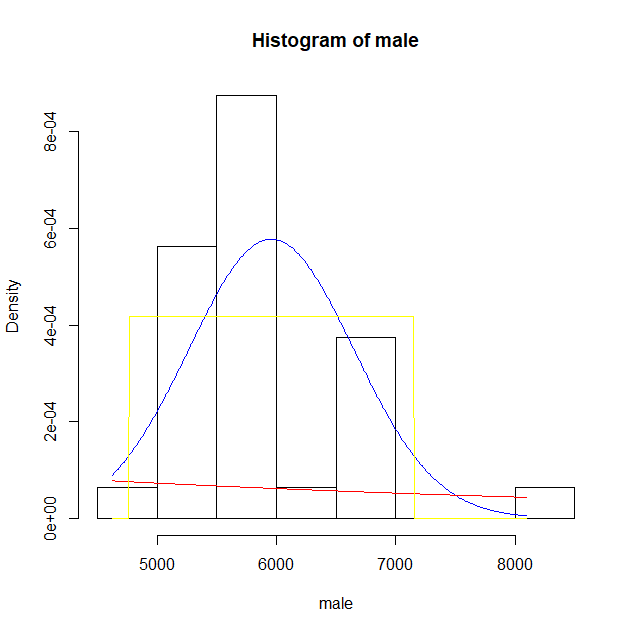
\includegraphics[width=0.4\textwidth]{porovnani-male.png} }}%
    \qquad
    \subfloat[Female]{{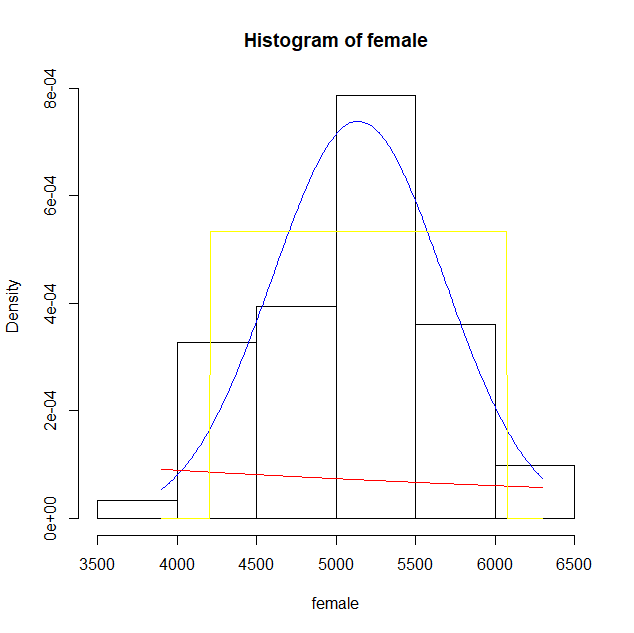
\includegraphics[width=0.4\textwidth]{porovnani-female.png} }}%
    \caption{Porovnání rozdělení}%
    \label{fig:example}%
\end{figure}
Došli jsme k záveru, že se u obou datasetu jedná o Normální rozdělení.

\subsection{Úkol číslo 4}
(1b) Pro každou skupinu zvlášť vygenerujte náhodný výběr o 100 hodnotách z rozdělení, které jste zvolili jako nejbližší, 
s parametry odhadnutými v předchozím bodě. Porovnejte histogram simulovaných hodnot s pozorovanými daty.
\begin{itemize}
	\item Male
		\begin{itemize}
			\item >> maleRand100 = rnorm(100, mean(male), sd(male))
				\begin{itemize}
				\item vybereme 100 náhodných hodnot použitím funkce rnorm
				\end{itemize}
			\item >> hist(maleRand100)
				\begin{itemize}
				\item vykreslíme z náhodně vybraných dat histogram
				\end{itemize}
		\end{itemize}
	\item Female
		\begin{itemize}
			\item >> femaleRand100 = rnorm(100, mean(female), sd(female))
				\begin{itemize}
				\item vybereme 100 náhodných hodnot použitím funkce rnorm
				\end{itemize}
			\item >> hist(femaleRand100)
				\begin{itemize}
				\item vykrelslíme z náhodně vybraných dat histogram 
				\end{itemize}
		\end{itemize}
\end{itemize}
\newpage
Výsledkem jsou následujíci grafy:
\begin{figure}[H]
  \centering
  \subfloat[Male]{
\includegraphics[width=0.4\textwidth]{nahodene100-male.png}}
  \qquad
  \subfloat[Female]{
\includegraphics[width=0.4\textwidth]{nahodene100-female.png}}
  \caption{Vygenerované histogramy}
\end{figure}
Došli jsme k závěru, že zatímco vygenrovaný graf pro male \iffalse fakt nevim jak to nazvat \fi se velmi liší od původního
histogramu což je způsobeno malým množstvím dat. U female \iffalse ¯\_(ツ)_/¯ \fi kde máme $\approx$ 2x více dat se histogramy
velmi podobají i přes relativně malé množství dat.

\subsection{Úkol číslo 5}
(1b) Pro každou skupinu zvlášť spočítejte oboustranný 95\% konfidenční interval pro střední hodnotu.

\begin{itemize}
	\item >> 
	working on it
	\begin{itemize}
		\item working on it
	\end{itemize}
\end{itemize}

%%% End document
\end{document}
